\section{Virus\-Bit\-Flip$<$ Fit\-T $>$ Class Template Reference}
\label{class_virus_bit_flip}\index{VirusBitFlip@{VirusBitFlip}}
Virus\-Bit\-Flip --$>$ changes 1 bit.  


{\tt \#include $<$Virus\-Op.h$>$}

Inheritance diagram for Virus\-Bit\-Flip$<$ Fit\-T $>$::\begin{figure}[H]
\begin{center}
\leavevmode
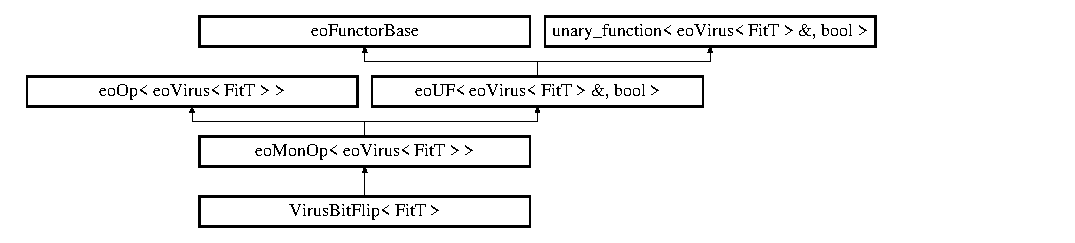
\includegraphics[height=2.81761cm]{class_virus_bit_flip}
\end{center}
\end{figure}
\subsection*{Public Member Functions}
\begin{CompactItemize}
\item 
virtual std::string {\bf class\-Name} () const \label{class_virus_bit_flip_a0}

\begin{CompactList}\small\item\em The class name. \item\end{CompactList}\item 
bool {\bf operator()} (eo\-Virus$<$ {\bf Fit\-T} $>$ \&\_\-chrom)
\begin{CompactList}\small\item\em Change one bit. \item\end{CompactList}\end{CompactItemize}


\subsection{Detailed Description}
\subsubsection*{template$<$class Fit\-T$>$ class Virus\-Bit\-Flip$<$ Fit\-T $>$}

Virus\-Bit\-Flip --$>$ changes 1 bit. 



Definition at line 40 of file Virus\-Op.h.

\subsection{Member Function Documentation}
\index{VirusBitFlip@{Virus\-Bit\-Flip}!operator()@{operator()}}
\index{operator()@{operator()}!VirusBitFlip@{Virus\-Bit\-Flip}}
\subsubsection{\setlength{\rightskip}{0pt plus 5cm}template$<$class Fit\-T$>$ bool {\bf Virus\-Bit\-Flip}$<$ {\bf Fit\-T} $>$::operator() (eo\-Virus$<$ {\bf Fit\-T} $>$ \& {\em \_\-chrom})\hspace{0.3cm}{\tt  [inline, virtual]}}\label{class_virus_bit_flip_a1}


Change one bit. 

\begin{Desc}
\item[Parameters:]
\begin{description}
\item[{\em chrom}]The cromosome which one bit is going to be changed. \end{description}
\end{Desc}


Implements {\bf eo\-UF$<$ eo\-Virus$<$ Fit\-T $>$ \&, bool $>$} {\rm (p.\,\pageref{classeo_u_f_a1})}.

Definition at line 49 of file Virus\-Op.h.

The documentation for this class was generated from the following file:\begin{CompactItemize}
\item 
Virus\-Op.h\end{CompactItemize}
